\documentclass{beamer} 
\usepackage{amsmath,amsthm}
\usepackage{graphicx,microtype,parskip}
\usepackage{caption,subcaption,multirow}
\usepackage{attrib}

\frenchspacing

\usetheme{default}
\usecolortheme{whale}

\setbeamertemplate{navigation symbols}{}

\setbeamercolor{title}{fg=blue,bg=white}

\setbeamercolor{block title}{fg=white,bg=gray}
\setbeamercolor{block body}{fg=black,bg=lightgray}

\setbeamercolor{block title alerted}{fg=white,bg=darkgray}
\setbeamercolor{block body alerted}{fg=black,bg=lightgray}


\title{How macroecology affects macroevolution}
\subtitle{the interplay between extinction intensity and trait-dependent extinction in brachiopods}
\author{Peter D Smits}
\institute{Committee on Evolutionary Biology, University of Chicago}
\titlegraphic{
  
\includegraphics[width=2.75cm,height=2.75cm,keepaspectratio=true]{figure/paleodb}
  \hspace*{0.35\paperwidth}
  
\includegraphics[width=2cm,height=2cm,keepaspectratio=true]{figure/chicago}
}
\date{}

\begin{document}

\begin{frame}
  \maketitle
\end{frame}

\begin{frame}
  \begin{block}{Selection on species traits}
    \begin{itemize}
      \item A species with a beneficial trait should persist for longer, on average, than a species without that beneficial trait \\{\footnotesize{(Jablonski 2008 \textit{Paleobio}, Rabosky and McCune 2010 \textit{TREE}).}}
      \item Taxon survival an aspect of \alert{taxon fitness} \\{\footnotesize{(Cooper 1984 \textit{J. Theo. Biol.}, Palmer and Feldman 2012 \textit{PLoS One}).}}
    \end{itemize}
  \end{block}
\end{frame}

\begin{frame}
  \begin{block}{Trait-dependent extinction}
    \begin{itemize}
      \item Extinction is second only to speciation in shaping diversity \\{\footnotesize{(Raup 1994 \textit{PNAS}, Stanley 1975 \textit{PNAS}).}}
      \item two major approaches: \alert{phylogenetic comparative} and \alert{paleobiological}
      \item difficult to estimate from phylogenies alone \\{\footnotesize{(Rabosky 2010 \textit{Evolution}, Liow et al 2010 \textit{Syst Biol}, Quental and Marshall 2008 \textit{Evolution}).}}
      \item fossil record is (imperfect) observation of extinction
    \end{itemize}
  \end{block}
\end{frame}

\begin{frame}
  \begin{alertblock}{Observation}
    At K/Pg mass extinction, biological traits (except geographic range) have no effect on \alert{bivalve} taxonomic survival.

    \attrib{\footnotesize{Jablonski, 1986, \em{Science}}}
  \end{alertblock}
\end{frame}

\begin{frame}
  \begin{alertblock}{Questions and analysis}
    \begin{itemize}
      \item How do the effect of emergent traits on duration (\alert{extinction selectivity}) vary with expected duration (\alert{extinction intensity})?
      \item \textbf{Approach:} hierarchical Bayesian survival model; \\effect estimates vary with origination cohort; \\correlation btw effects modeled.
    \end{itemize}
  \end{alertblock}
\end{frame}

\begin{frame}
  \frametitle{Intensity and selectivity}
  \begin{center}
    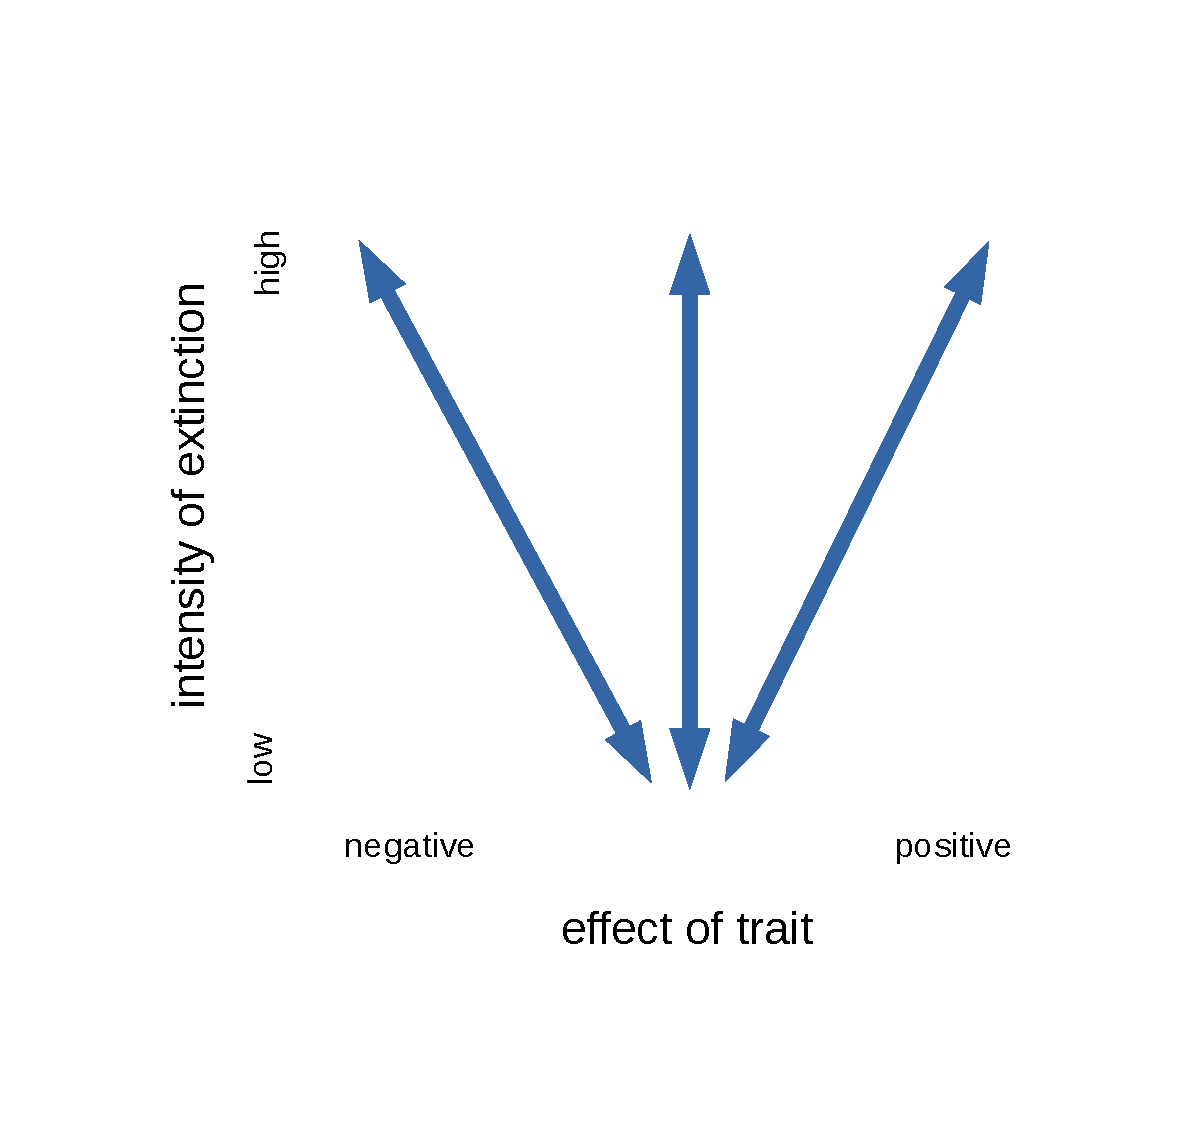
\includegraphics[width = \textwidth,height = 0.8\textheight,keepaspectratio = true]{figure/intensity_selectivity_base}
  \end{center}
\end{frame}

\begin{frame}
  \frametitle{Brachiopods}
  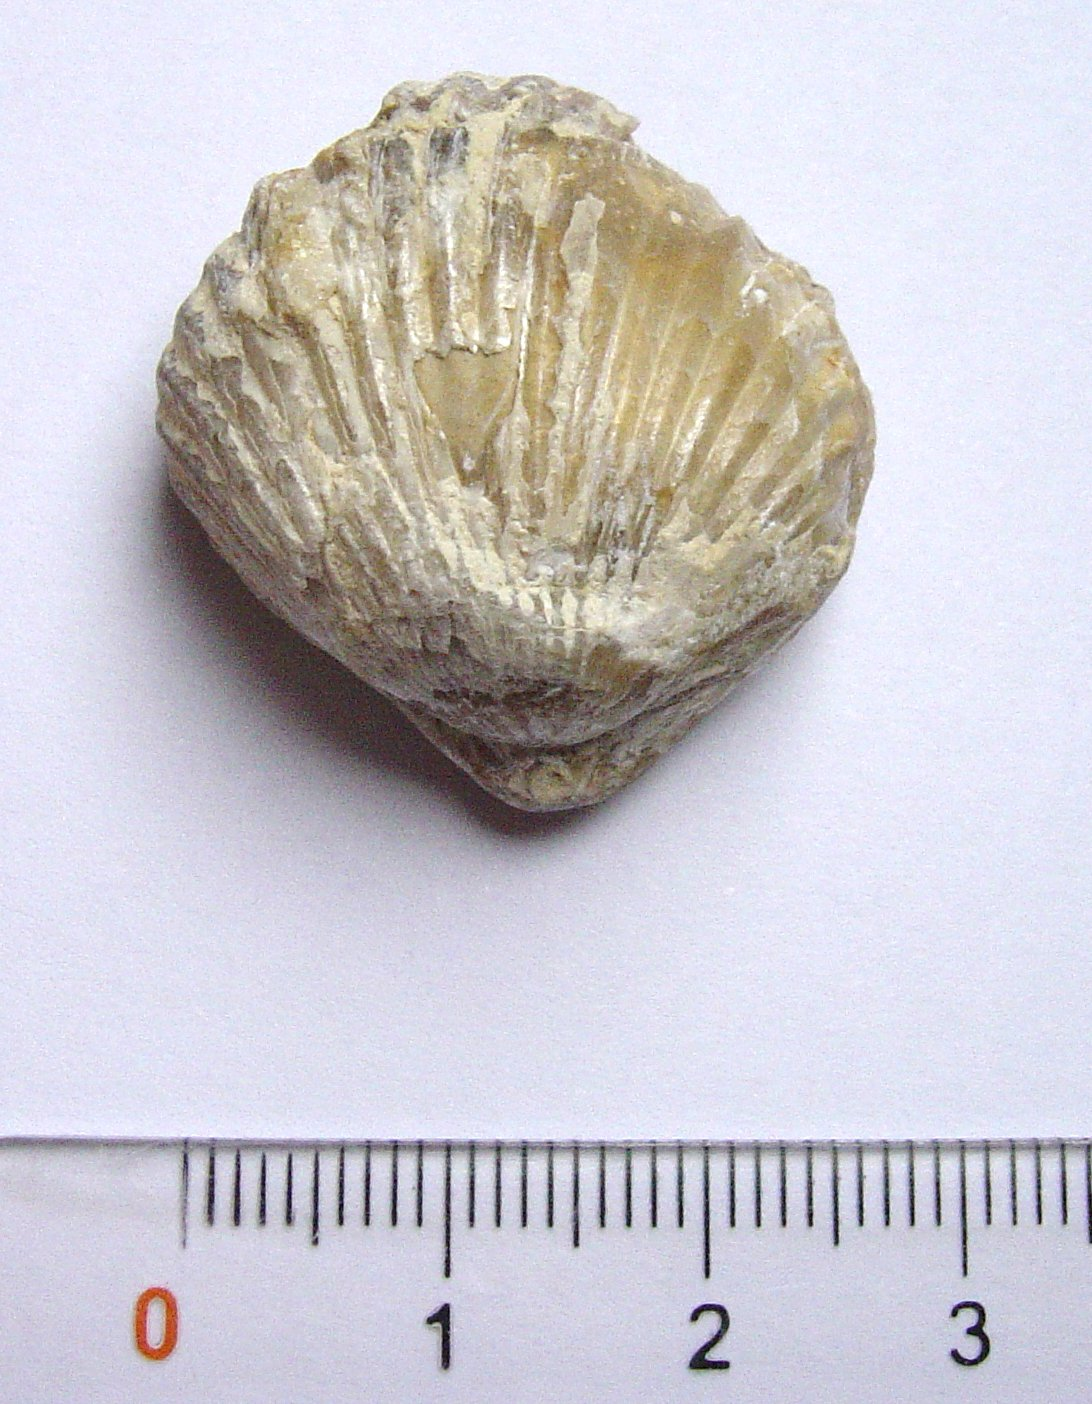
\includegraphics[width = 0.45\textwidth,height = 0.8\textheight,keepaspectratio = true]{figure/Brachiopod_fossil}
  \includegraphics[width = 0.45\textwidth,height = 0.8\textheight,keepaspectratio = true]{figure/Burmirhynchionella_decorata_brachial_CRF}

  \tiny{\attrib{ComputerHotline, wikimedia CC BY 2.5; Dwergenpaartje, wikimedia CC BY-SA 3.0}}
\end{frame}

\begin{frame}
  \frametitle{Post-Cambrian Paleozoic brachiopod genera and covariates}
  \begin{itemize}
    \item time range approx. 488-252 Mya.
    \item stage as time unit; duration measured in stages (2-5 My each)
    \item multiple emergent traits analyzed; estimates vary by origination cohort
      \begin{itemize}
        \item geographic range
        \item body size
        \item environmental preference (v, v\(^2\))
      \end{itemize}
    \item gap statistic as measure of sampling {\footnotesize{(Foote and Raup 1996 \textit{Paleobio})}} \\imputed for taxa with short durations
  \end{itemize}
\end{frame}

\begin{frame}
  \frametitle{Hypothesis of effect of geographic range}
  \begin{center}
    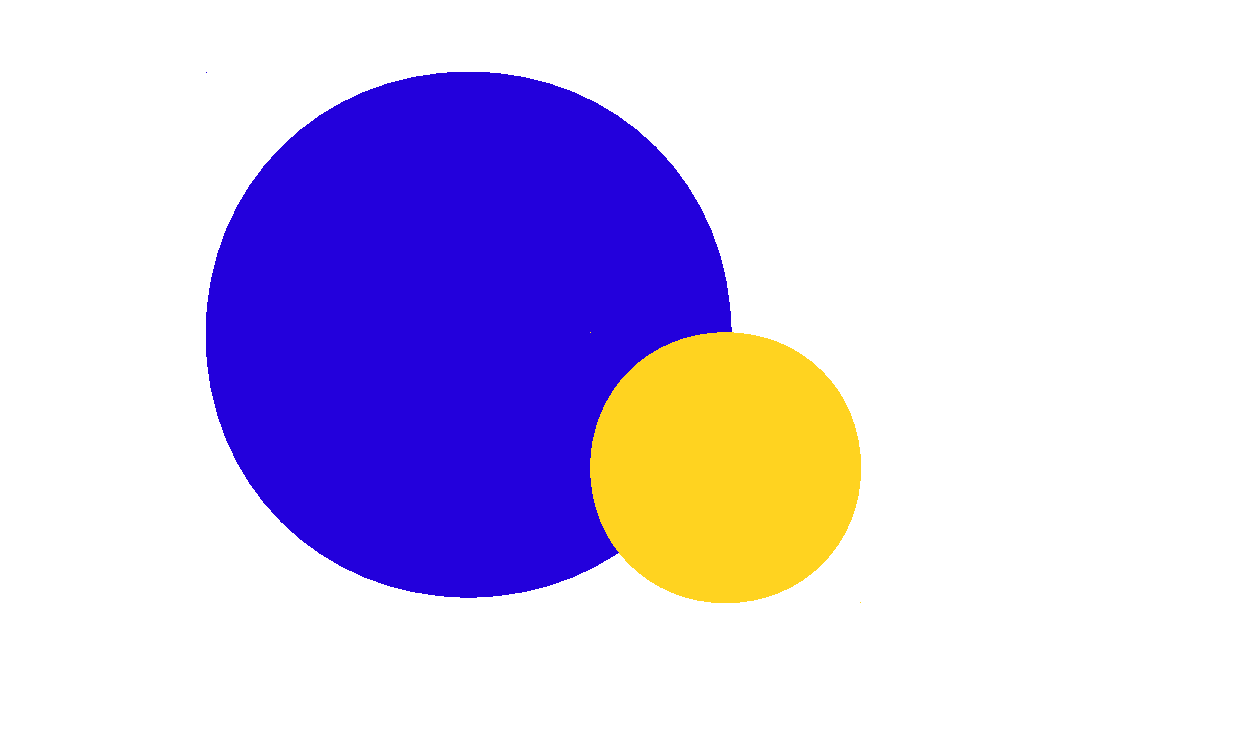
\includegraphics[width = \textwidth,height = 0.8\textheight,keepaspectratio = true]{figure/geo_range_1}
  \end{center}
\end{frame}

\begin{frame}
  \frametitle{Hypothesis of effect of geographic range}
  \begin{center}
    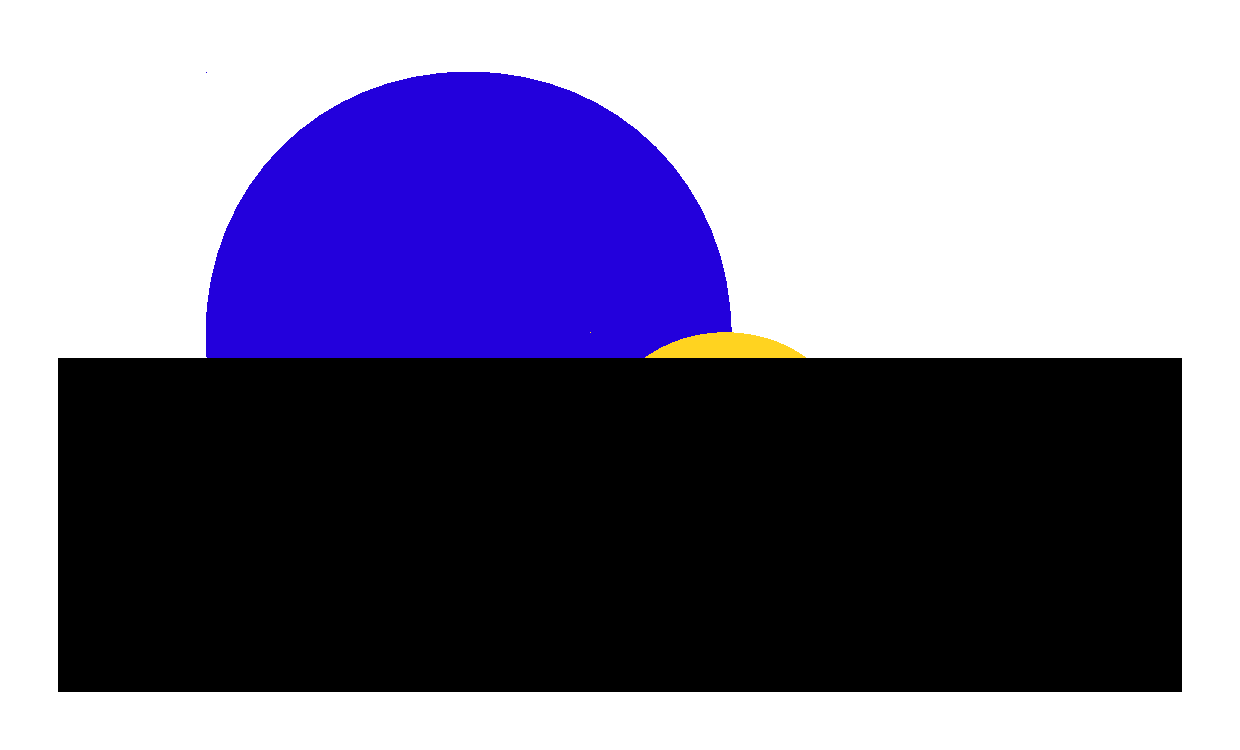
\includegraphics[width = \textwidth,height = 0.8\textheight,keepaspectratio = true]{figure/geo_range_2}
  \end{center}
\end{frame}


\begin{frame}
  \frametitle{Hypotheses of effect of environmental preference}
  \begin{quote}
    When related phyla die out \dots more specialized phyla tend to become extinct before less specialized. This phenomenon is also far from universal, but it is so common that it does deserve recognition as a rule or principle in evolutionary studies: \textbf{the rule of the survival of the relatively unspecialized.}

    \attrib{\footnotesize{Simpson, 1944, \em{Tempo and Mode in Evolution}, p. 143}}
  \end{quote}
\end{frame}

\begin{frame}
  \frametitle{Hierarchical survival model}
  \begin{center}
    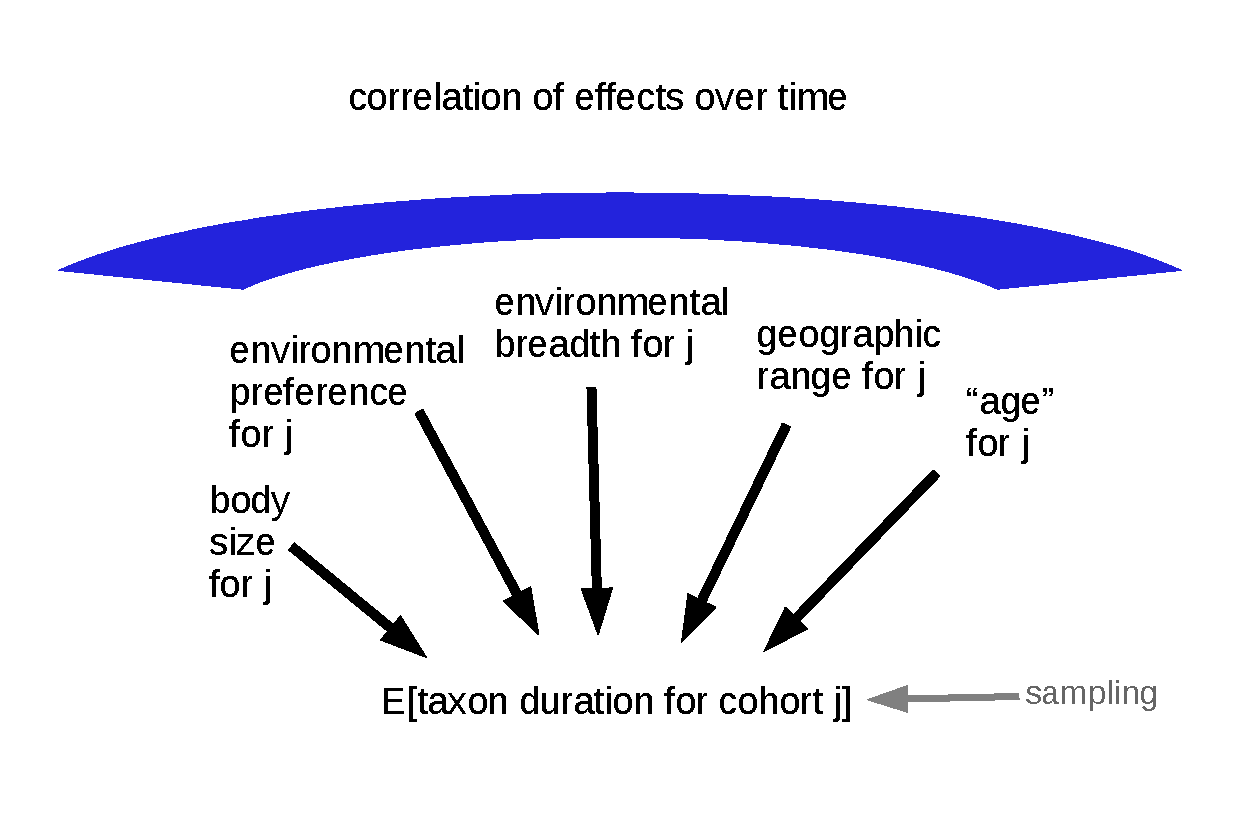
\includegraphics[width = \textwidth,height = 0.8\textheight,keepaspectratio = true]{figure/simple_model}
  \end{center}
\end{frame}

\begin{frame}
  \frametitle{Variation in trait effects between cohorts}

  \begin{center}
    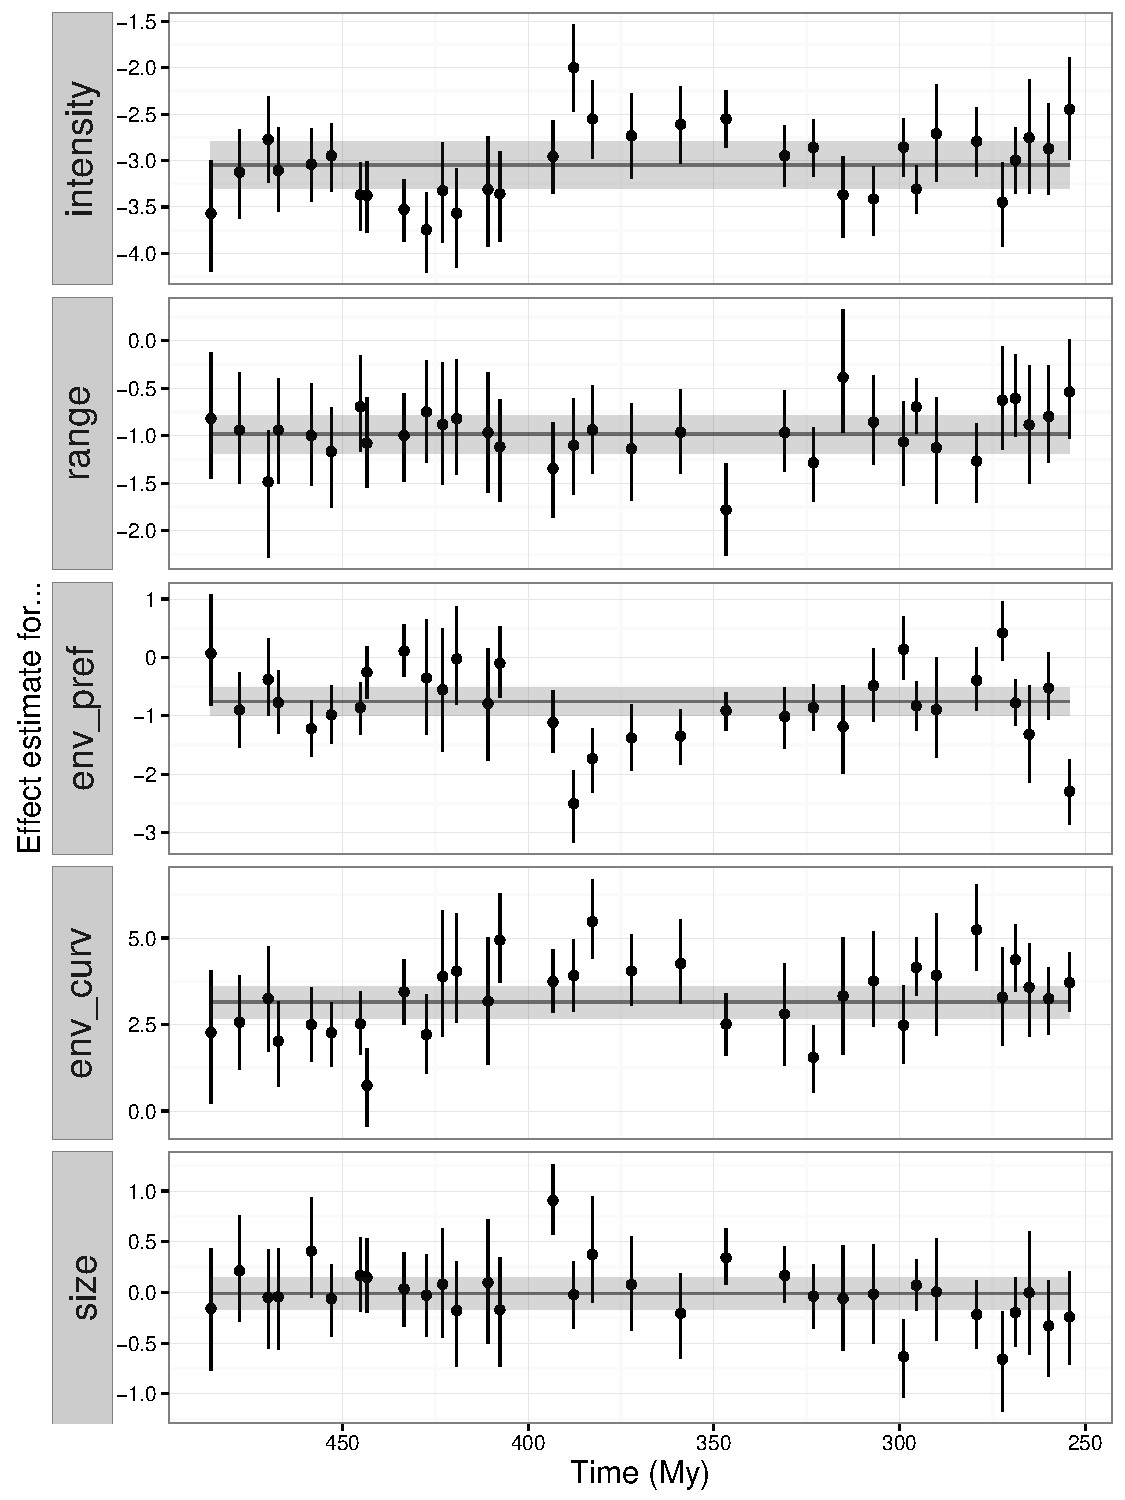
\includegraphics[width = \textwidth,height = 0.8\textheight,keepaspectratio = true]{figure/cohort_series}
  \end{center}
\end{frame}

\begin{frame}
  \frametitle{Overall effect of environmental preference}

  \begin{center}
    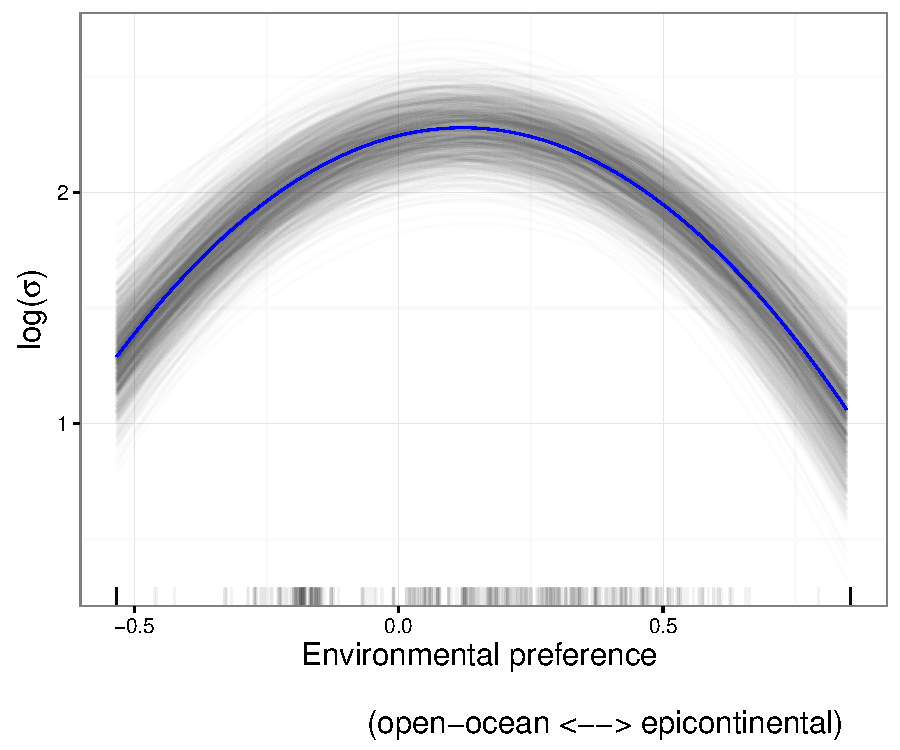
\includegraphics[width = \textwidth,height = 0.8\textheight,keepaspectratio = true]{figure/env_effect}
  \end{center}
\end{frame}

\begin{frame}
  \frametitle{Change in effect of environment between cohorts}

  \begin{center}
    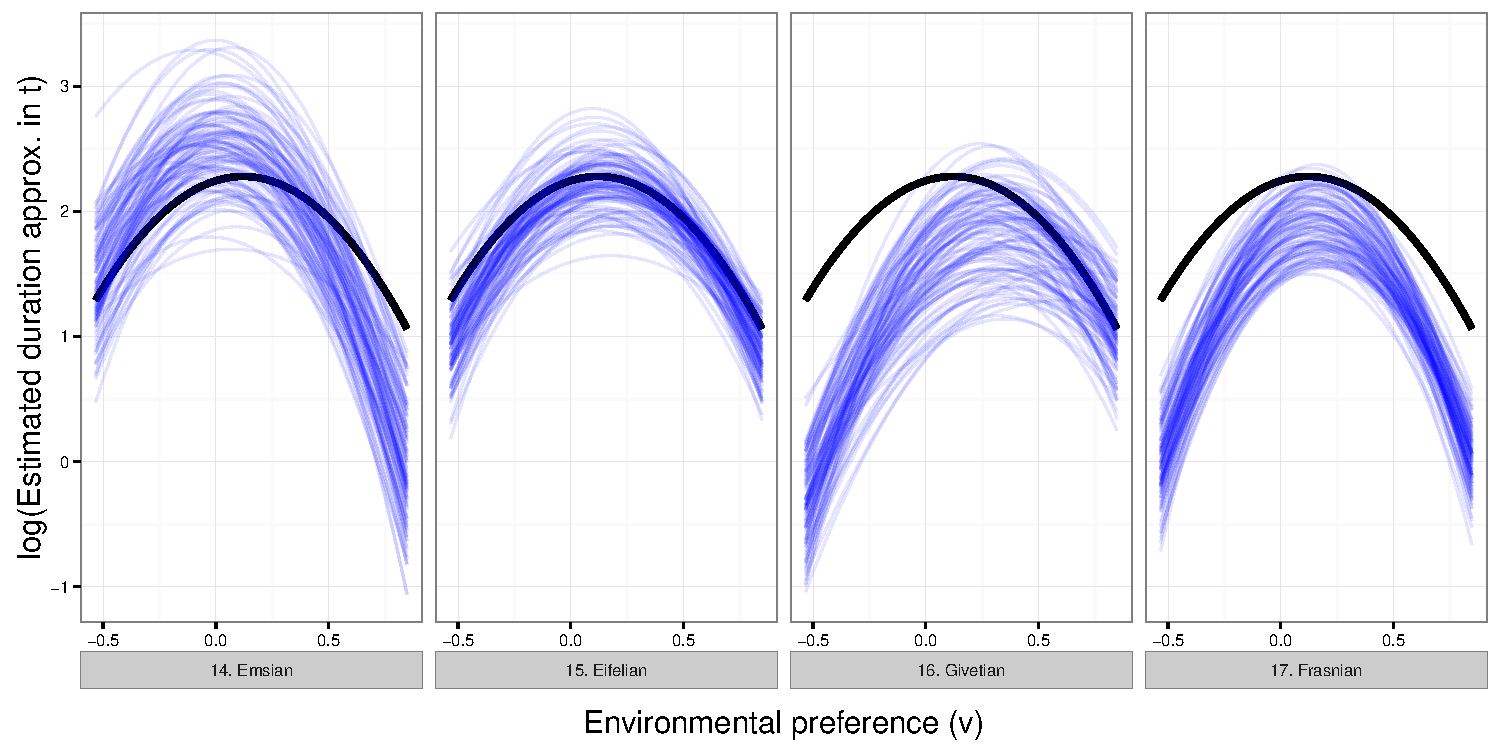
\includegraphics[width = \textwidth,height = 0.8\textheight,keepaspectratio = true]{figure/env_cohort_short}
  \end{center}
\end{frame}

\begin{frame}
  \frametitle{Change in effect of environment between cohorts}

  \begin{center}
    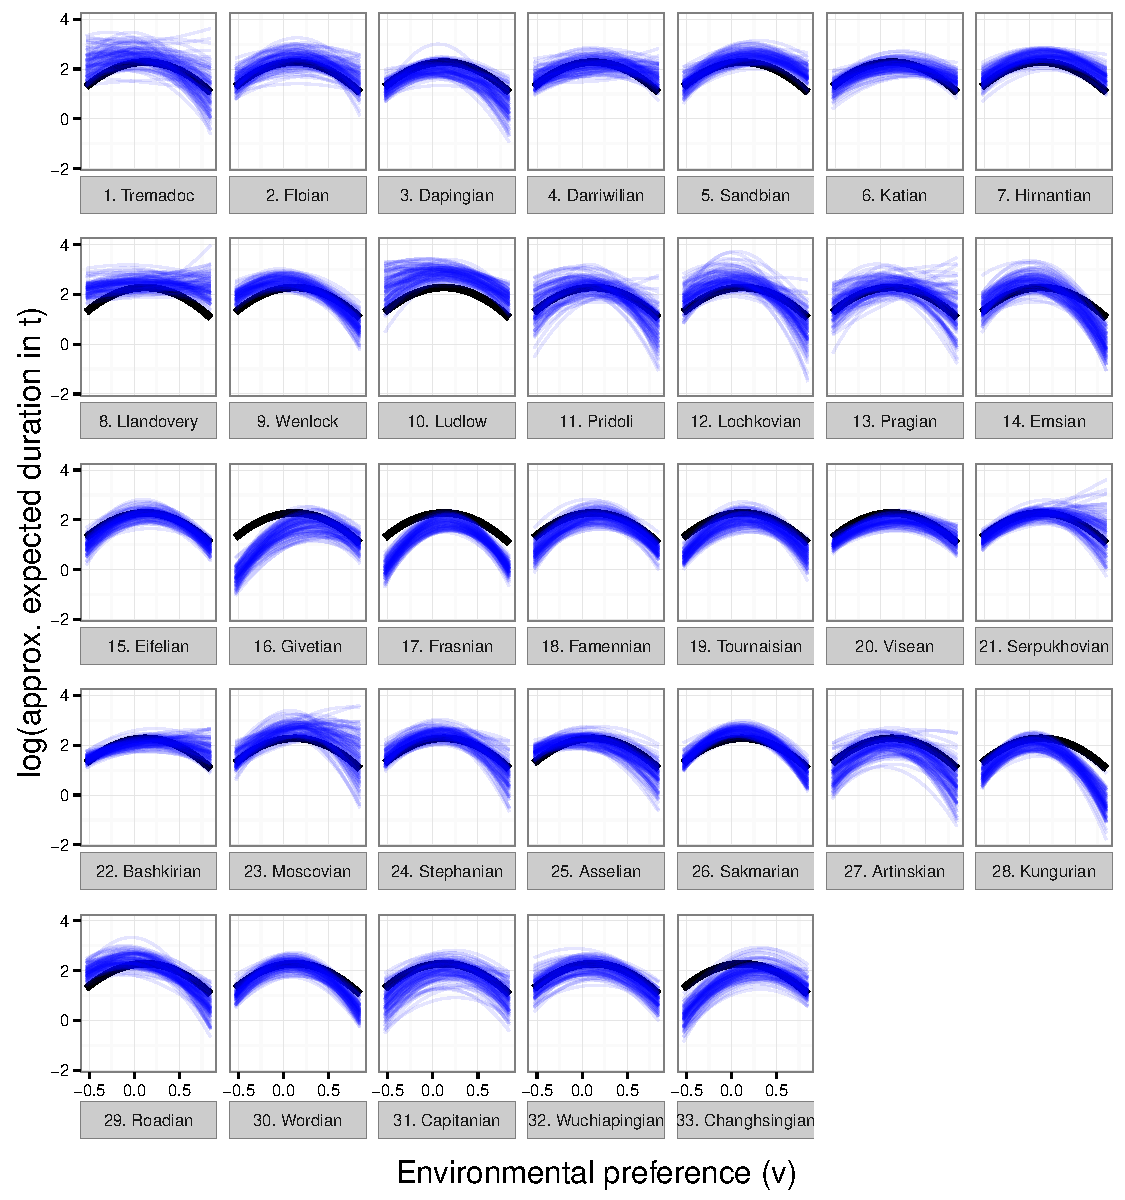
\includegraphics[width = 0.8\textwidth,height = 0.8\textheight,keepaspectratio = true]{figure/env_cohort}
  \end{center}
\end{frame}

\begin{frame}
  \frametitle{Correlation of effects between cohorts}

  \begin{center}
    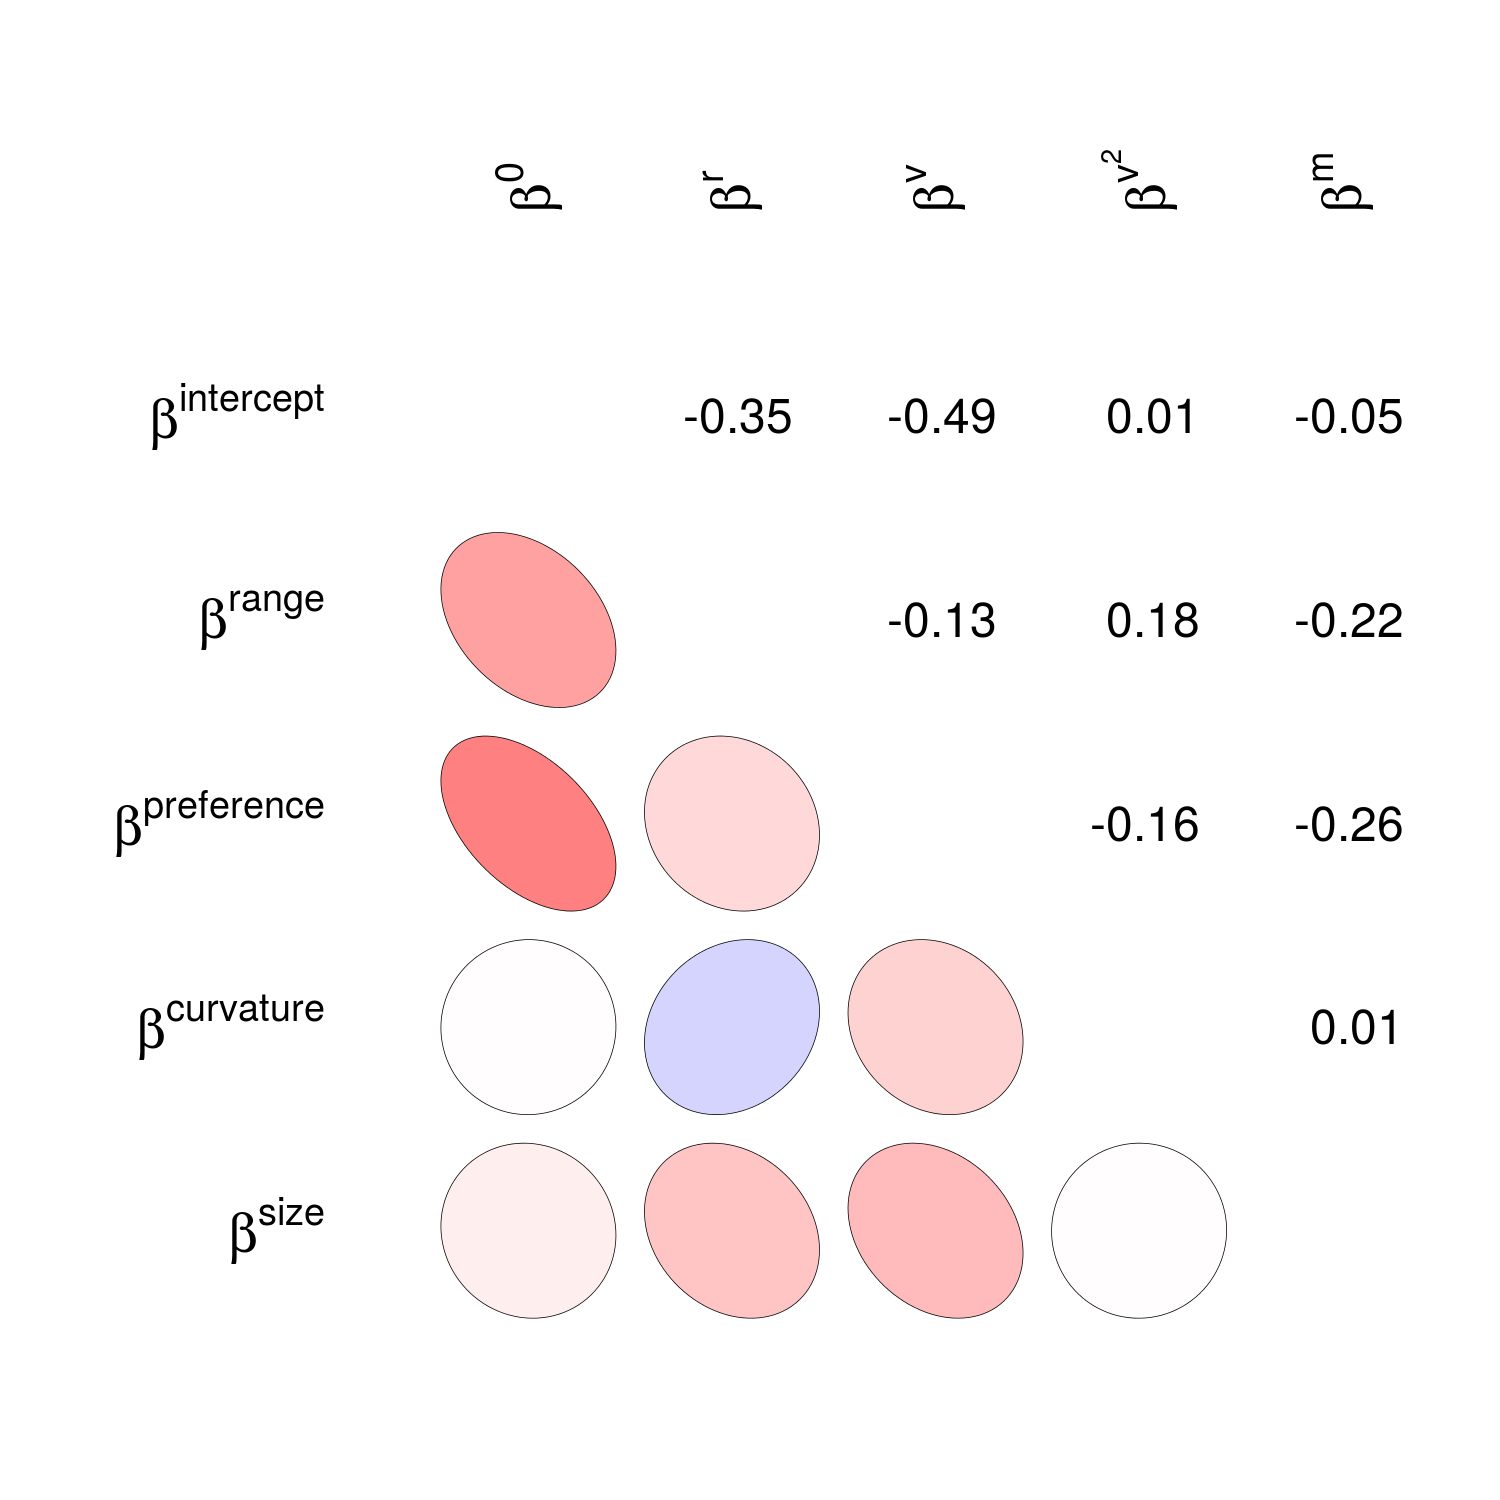
\includegraphics[width = \textwidth,height = 0.9\textheight,keepaspectratio = true]{figure/wei_cor_heatmap}
  \end{center}
\end{frame}

\begin{frame}
  \begin{block}{Effect summary}
    \begin{itemize}
      \item Effect of geographic range consistent with prior expectations; low variance.
      \item No effect of body size; low variance.
      \item Epicontinental environmental preference slightly favored on averaged; high variance. 
      \item Strong support for survival of unspecialized as generalization wrt environmental preference; medium variance.
    \end{itemize}
  \end{block}
\end{frame}

\begin{frame}
  \begin{alertblock}{Macroevolutionary process}
    \begin{itemize}
      \item Magnitude of effect of geographic range and environmental preference increase with extinction intensity.
      \item As extinction risk decreases, the differences between taxa matter less.
    \end{itemize}
  \end{alertblock}
\end{frame}

\begin{frame}
  \frametitle{Acknowledgements}
  \begin{columns}
    \begin{column}{0.5\textwidth}
      \begin{itemize}
        \item Advising
          \begin{itemize}
            \item Kenneth D. Angielczyk, Michael J. Foote, \\P. David Polly, \\Richard H. Ree, \\Graham Slater
          \end{itemize}
        \item Angielczyk Lab
          \begin{itemize}
            \item {\small{David Grossnickle, \\Dallas Krentzel, \\Jackie Lungmus}}
          \end{itemize}
        \item Foote lab
          \begin{itemize}
            \item {\small{Marites Villarosa Garcia, \\Nadia Pierrehumbert}}
          \end{itemize}
      \end{itemize}
    \end{column}
    \begin{column}{0.5\textwidth}
      \begin{itemize}
        \item {\footnotesize{Stewart Edie, \\Elizabeth Sander, \\Laura Southcott, \\Courtney Stepien}}
        \item {\footnotesize{David Bapst, \\Ben Frable, \\\textbf{Arnold Miller}, \\Peter Wagner}}
        \item {\footnotesize{UChicago CEB, Sandy Carlson }}
      \end{itemize}

      \vspace*{0.05\textheight}
      \begin{center}
        
\includegraphics[height=0.2\textheight,width=\textwidth,keepaspectratio=true]{figure/paleodb}
      \end{center}
    \end{column}
  \end{columns}
\end{frame}

\appendix

\begin{frame}
  \frametitle{Model adequacy}
  \begin{columns}
    \begin{column}{0.5\textwidth}
      \begin{center}
        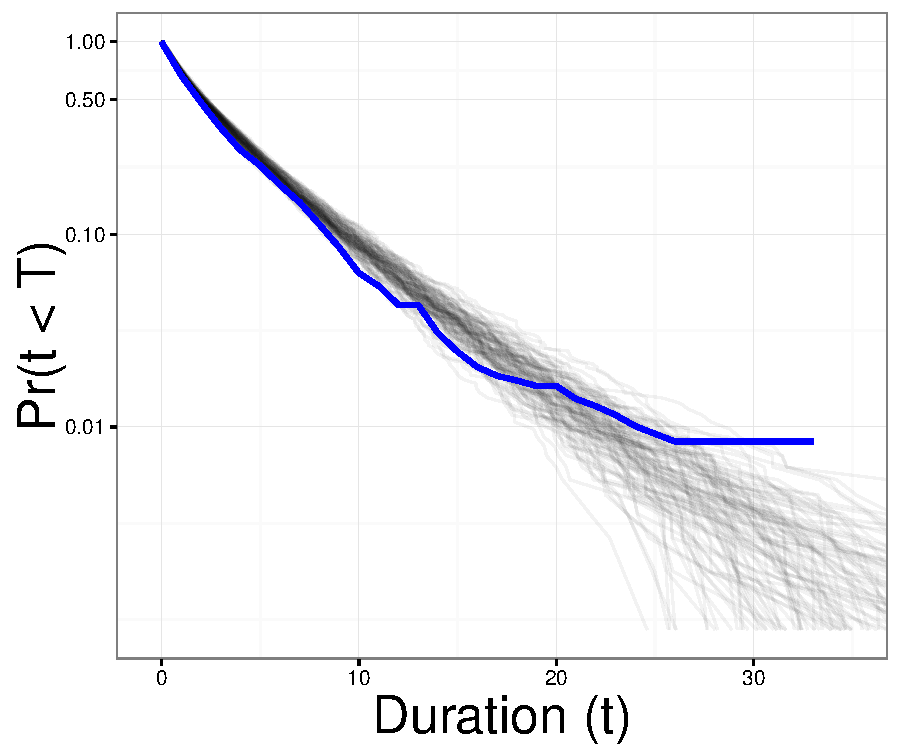
\includegraphics[width=\textwidth,height=0.8\textheight,keepaspectratio=true]{figure/survival_curves}
      \end{center}
    \end{column}
    \begin{column}{0.5\textwidth}
      \begin{center}
        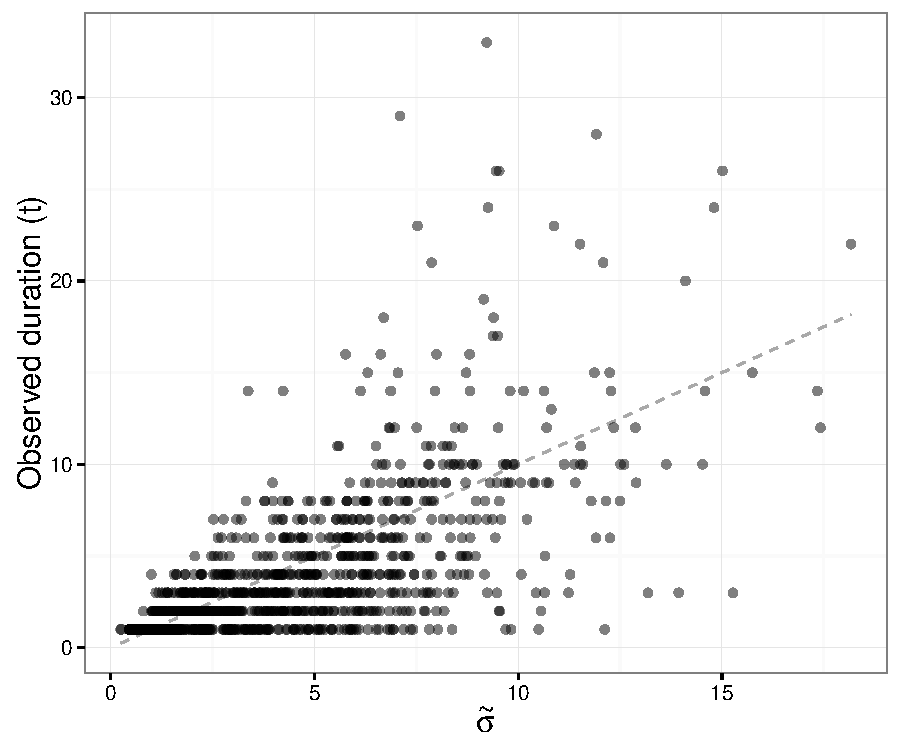
\includegraphics[width=\textwidth,height=0.8\textheight,keepaspectratio=true]{figure/shotgun}
      \end{center}
    \end{column}
  \end{columns}
\end{frame}

\begin{frame}
  \begin{block}{New measure of taxon's environmental affinity}
    (\# epicontinental / total \# occurrences) is what quantile of the distribution of all other background occurrences Beta(\(\alpha\), \(\beta\)).
    \begin{itemize}
      \item \(\alpha\) is the \# epicontinental background occurrences (+ 1).
      \item \(\beta\) is the \# open ocean background (+ 1).
    \end{itemize}
  \end{block}
\end{frame}


\begin{frame}
  \begin{block}{Measure of sampling and imputed values}
    Sampling is measured as the gap statistic \(r\): \\(number of bins with an occurrence - 2) / (duration in bins - 2)

    Can only be estimated for taxa with duration of three or more. \\Have to impute (e.g. fill-in) the values for all other taxa \(r^{\ast}\).
    \begin{align*}
      s &\sim \text{Beta}(\phi, \lambda) \\
      \phi &= \text{logit}^{-1}(W\gamma) \\
      s^{\ast} &\sim \text{Beta}(\phi^{\ast}, \lambda) \\
      \phi^{\ast} &= \text{logit}^{-1}(W^{\ast}\gamma) \\
    \end{align*}
    \scriptsize{Note: Beta distribution parameterized in terms of mean \(\phi\) and total count \(\lambda\). \\Also, this presentation excludes final (hyper)priors.}
  \end{block}
\end{frame}


\begin{frame}
  \frametitle{Sampling statement for the joint posterior probability}

  \begin{columns}
    \begin{column}{0.5\textwidth}
      \begin{align*}
        y_{i, t} &\sim \text{Weibull}(\sigma_{i, t}, \alpha) \\
        \log(\sigma_{i, t}) &= \frac{X_{i}B_{j[i], t} + \delta s_{i}}{\alpha} \\
        B_{j} &\sim \text{MVN}(\mu, \Sigma) \\
        \Sigma &= \text{diag}(\tau) \Omega \text{diag}(\tau) \\
        s_{i} &\sim \text{Beta}(\phi_{i}, \lambda) \\
        \phi_{i} &= \text{logit}^{-1}(W_{i}\gamma) \\
      \end{align*}
    \end{column}
    \begin{column}{0.5\textwidth}
      \begin{align*}
        \mu_{intensity} &\sim \mathcal{N}(0, 5) \\
        \mu_{range} &\sim \mathcal{N}(-1, 1) \\
        \mu_{env pref} &\sim \mathcal{N}(0, 1) \\
        \mu_{env curve} &\sim \mathcal{N}(1, 1) \\
        \mu_{size} &\sim \mathcal{N}(0, 1) \\
        \delta &\sim \mathcal{N}(0, 1) \\
        \tau &\sim \text{C}^{+}(1) \\
        \Omega &\sim \text{LKJ}(1) \\
        \lambda &\sim \text{Pareto}(0.1, 1.5) \\
        \gamma &\sim \mathcal{N}(0, 1) \\
      \end{align*}
    \end{column}
  \end{columns}

  \scriptsize{Note: Calculation of log probability of right and left censored observations is modified from the above}
\end{frame}


\begin{frame}
  \frametitle{Inspecting the imputations}
  \begin{center}
    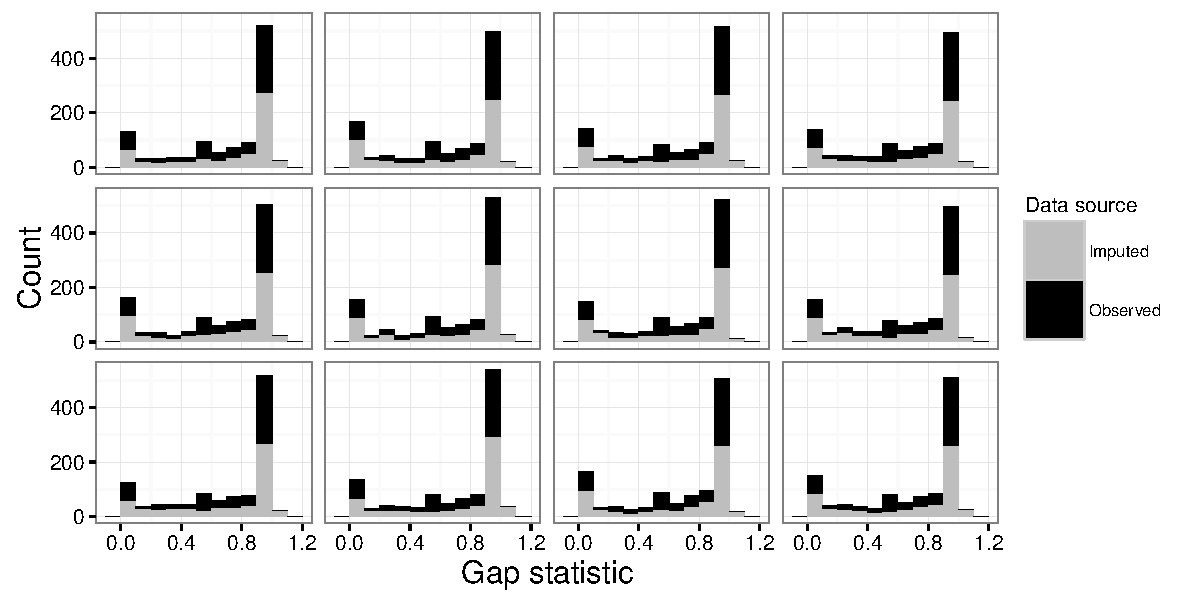
\includegraphics[width=\textwidth,height=0.8\textheight,keepaspectratio=true]{figure/imputation_compare}
  \end{center}
\end{frame}


\end{document}
